La segunda propuesta se aplica en el campo de optimización multi-objetivo y está basada en la extensión del operador de
cruce \SBX{}.
%
En esta sección se introducen, en primer lugar, varios conceptos relacionados con los algoritmos evolutivos multi-objetivo, 
para posteriormente describir algunas de las clasificaciones más populares de operadores de cruce.
%
Finalmente, se realiza un análisis del operador \SBX{} y en base al mismo se propone una variante dinámica denominada 
\textit{Operador de Cruce Dinámico basado en Simulación Binaria} (Dynamic Simulated Binary Crossover - \DSBX{}), el cual
es validado experimentalmente.

\subsection{Algoritmos evolutivos multi-objetivo}

Los \EAS{} han sido utilizados frecuentemente para lidiar con problemas de optimización multi-objetivo (Multi-objective Optimization Problems - MOPs).
%
Particularmente, Un MOP continuo basado en minimización puede ser definido como se indica en la Ecuación (\ref{eqn:Model_general}) de la sección~\ref{sec:Introduction}, fijando la $M$
a un valor mayor que uno.
%
Dadas dos soluciones $\vec{x}$, $\vec{y}$ $\in \Omega$, $\vec{x}$ domina a $\vec{y}$, denotado por $\vec{x} \prec \vec{y}$, 
si y solo si $\forall m \in {1,2,...,M} : f_m(x_i) \leq f_m(y_i)$ y $\exists m \in {1,2,...,M} : f_m(x_i) < f_m(y_i)$.
%
Una solución $\vec{x^*} \in \Omega$ es conocida como solución óptima de Pareto si no existe otra solución $\vec{x} \in \Omega$ que domine a $\vec{x^*}$.
%
El conjunto de Pareto es el conjunto de todas las soluciones óptimas de Pareto y el frente de Pareto está formado por las imágenes del conjunto de Pareto.
%
El propósito de un \textit{Algoritmo Evolutivo Multi-Objetivo} (Multi-objective Evolutionary Algorithm - MOEA) es, esencialmente, obtener 
un conjunto de soluciones bien distribuidas y cercanas a las soluciones del frente de Pareto.

En los últimos años, se han diseñado una gran cantidad de \MOEAS{} siguiendo distintos principios.
%
A raíz de esto se han propuesto varias taxonomías~\cite{Joel:BOOK_MOEAs} y, por ejemplo, en base a sus principios de diseño
se pueden clasificar en basados en la dominancia de Pareto, indicadores y/o descomposición~\cite{pilat2010evolutionary}.
%
Hay algoritmos muy competitivos de cada uno de los grupos por lo que en esta sección se consideraron \MOEAS{} de todos los grupos para realizar la validación.
%
Particularmente, la validación experimental se desarrolló incluyendo a los algoritmos \textit{Algoritmo Genético basado en Ordenación de los No-Dominados} 
(Non-Dominated Sorting Genetic Algorithm - NSGA-II)~\cite{Joel:NSGAII}, el \textit{MOEA basado en descomposición} (MOEA based on Decomposition - \MOEAD{})~\cite{Joel:MOEAD} 
y el \textit{Algoritmo Evolutivo Multi-objetivo basado en la Métrica-S} (the $S$-Metric Selection Evolutionary Multi-objective Optimization Algorithm - \SMSEMOA{})~\cite{Joel:SMSEMOA}.
%
Estos algoritmos son representativos de los basados en dominancia, basados en descomposición y basados en indicadores respectivamente.
%
%Las siguientes sub-secciones describen cada uno de los paradigmas involucrados en los métodos seleccionados.
%The following subsections briefly describe each one of these paradigms and introduce the selected methods.

%%%%\subsubsection{Algoritmos basados en el concepto de dominancia - NSGA-II }
%%%%%\subsubsection{Domination Based MOEAs - NSGA-II}
%%%%
%%%%Uno de los paradigmas mas reconocidos son los enfoques basados en dominancia.
%%%%%
%%%%Los \MOEAS{} que pertenecen a esta categoría se basan en la aplicación de la relación de dominancia para diseñar los distintos componentes de los mismos, especialmente en la fase de selección.
%%%%%
%%%%Dado que la relación de dominancia no promueve la diversidad de forma implícita en el espacio de los objetivos se han desarrollado técnicas para obtener una diversidad en el espacio de los objetivos como es el niching, crowding y/o clustering que usualmente se integran con el propósito de obtener una diversidad aceptable en el espacio de los objetivos.
%%%%%
%%%%Una debilidad importante en los métodos que están basados en la relación de dominancia, es la escalabilidad de la dimensionalidad en el espacio de los objetivos.
%%%%%
%%%%De hecho, conforme se incrementa el número de objetivos, la presión de selección se reduce significativamente.
%%%%%
%%%%A pesar de que se han desarrollado algunas estrategias para solventar este inconveniente \cite{horoba2008benefits}, este parece ser la debilidad mas importante de este tipo de algoritmos.
%%%%
%%%%El \NSGAII{} es uno de los algoritmos mas importantes de este grupo.
%%%%%
%%%%Este algoritmo~\cite{Joel:NSGAII} considera un operador de selección especial el cual está basado en los procedimientos de la ordenación de las soluciones no dominadas y en el amontonamiento (crowding).
%%%%%
%%%%Particularmente, el procedimiento que realiza la ordenación de las soluciones no dominadas se utiliza para proporcionar una convergencia hacia el frente de Pareto, mientras que el procedimiento de amontonamiento se utiliza para promover la diversidad en el espacio de los objetivos.
%%%%
%%%%\subsubsection{Algoritmos multi-objetivo basados en descomposición - MOEA/D}
%%%%
%%%%Los \MOEAS{} basados en descomposición \cite{Joel:MOEAD} transforman un \MOP{} en un conjunto de problemas de optimización mono-objetivo los cuales son resueltos simultáneamente.
%%%%%
%%%%Esta transformación se puede lograr a través de distintos enfoques.
%%%%%
%%%%La función pesada de Tchebycheff es quizás uno de los enfoque más importantes.
%%%%%
%%%%Específicamente, esta función requiere un conjunto de pesos bien distribuidos, esto con el propósito de alcanzar soluciones bien distribuidas a lo largo del frente de Pareto.
%%%%%
%%%%Sin embargo, este tipo de algoritmos poseen una desventaja importante, es decir los vectores de pesos dependen de la geometría que posee el frente de Pareto.
%%%%El \MOEA{}~\cite{Joel:MOEAD} es un \MOEA{} muy popular de los basados en descomposición.
%%%%%
%%%%Este incluye varias características, tales como la descomposición de los problemas, la agregación de los pesos con los objetivos y las restricciones de emparejamiento que están basadas en la definición de vecindarios.
%%%%%
%%%%El algoritmo \MOEADDE{} es considerado como una variante popular del \MOEAD{}, el cual utiliza operadores de \DE{}~\cite{price2006differential} y el operador de mutación polinomial~\cite{hamdan2012distribution} en la fase de reemplazo.
%%%%%
%%%%Adicionalmente, este algoritmo tiene dos mecanismos especiales para mantener la diversidad de la población~\cite{zhang2009performance}.
%%%%
%%%%\subsubsection{Algoritmos multi-objetivo basados en indicadores - SMS-EMOA}
%%%%
%%%%En optimización multi-objetivo se han desarrollado varios indicadores de calidad con el propósito de comparar el rendimiento de los \MOEAS{}.
%%%%%
%%%%Desde que estos indicadores miden la calidad de las aproximaciones obtenidas por los \MOEAS{}, se ha propuesto un paradigma basado en en la aplicación de estos indicadores.
%%%%%
%%%%Particularmente, los indicadores reemplazan a la relación de dominancia de Pareto con el propósito de guiar el proceso de optimización.
%%%%%
%%%%Principalmente, el hipervolumen es un indicador ampliamente aceptado por su relación completa de Pareto (Pareto-compliance)~\cite{Joel:IGDPlus_And_GDPlus}.
%%%%%
%%%%Una de la principales ventajas de estos algoritmos es que los indicadores normalmente consideran tanto la calidad de las soluciones como su diversidad, por lo tanto no se requieren mecanismos adicionales para preservar la diversidad.
%%%%
%%%%El \SMSEMOA{}~\cite{Joel:SMSEMOA} es un \MOEA{} popular basado en indicadores.
%%%%%
%%%%Este \MOEA{} es considerado como un algoritmo híbrido ya que utiliza tanto indicadores como el concepto de la dominancia de Pareto.
%%%%%
%%%%Esencialmente, este algoritmo integra el procedimiento para ordenar a las soluciones no dominadas con la métrica del hipervolumen.
%%%%%
%%%%Por lo tanto el \SMSEMOA{} aplica el hipervolumen como estimador de densidad el cual es computacionalmente complejo.
%%%%%
%%%%Particularmente, la fase de reemplazo elimina al individuo que pertenece al frente con peor rango y cuya contribución al hipervolumen sea mínima.
%%%%%
%%%%Debido a su comportamiento prometedor, el \SMSEMOA{} se ha considerado como parte de nuestra validación experimental.
%

\begin{figure}[!t]
\centering
%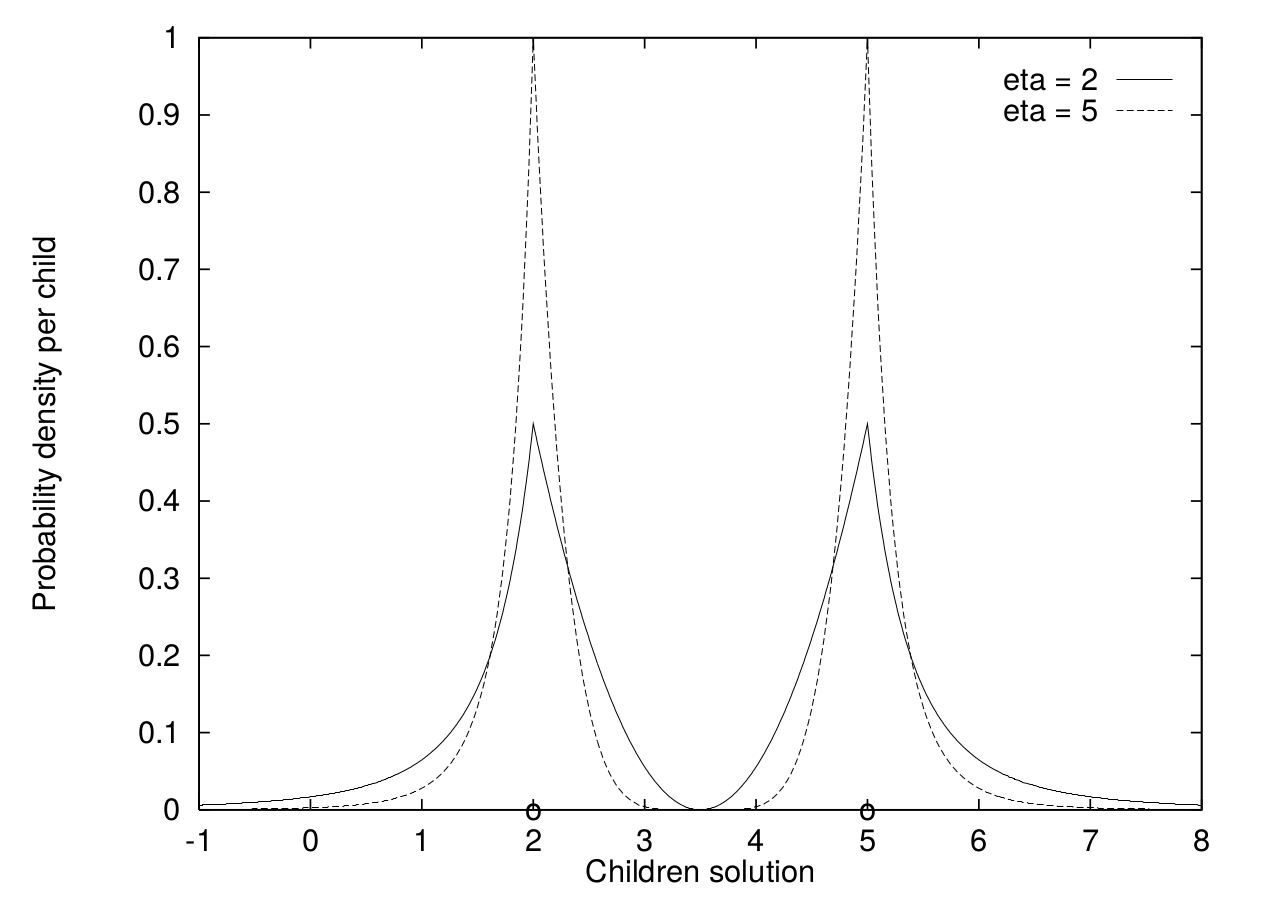
\includegraphics[width=2.5in]{img/Operadores/DensitySBX_English.png}
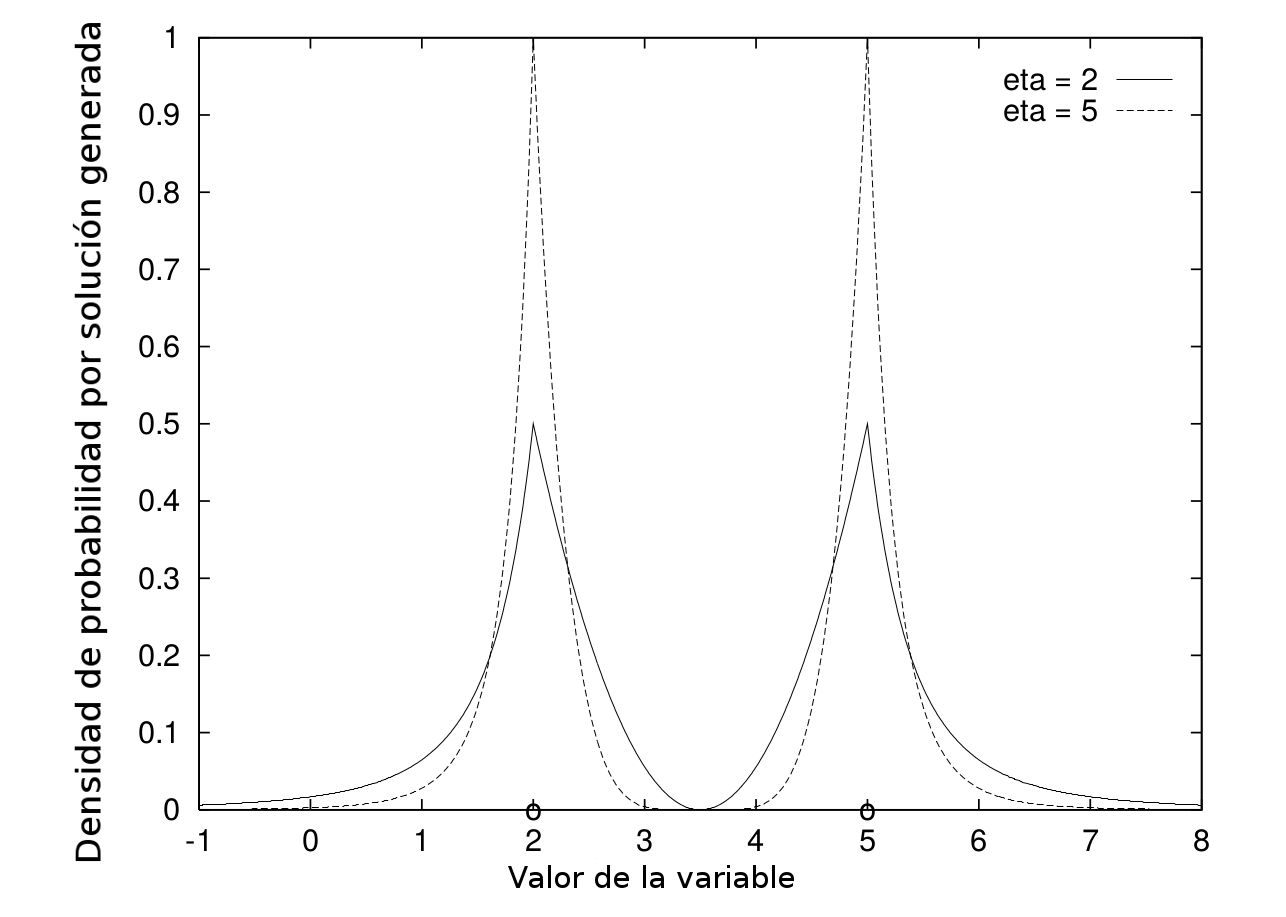
\includegraphics[width=0.5\textwidth]{img/Operadores/DensitySBX.png} 
\caption{Función de densidad del operador de cruce \SBX{} con índices de distribución $2$ y $5$. Las soluciones padre están ubicadas en $2$ y $5$ respectivamente.}
\label{fig:fig_sim}
\end{figure}

\begin{figure}[!t]
\centering
\begin{tabular}{cc}
   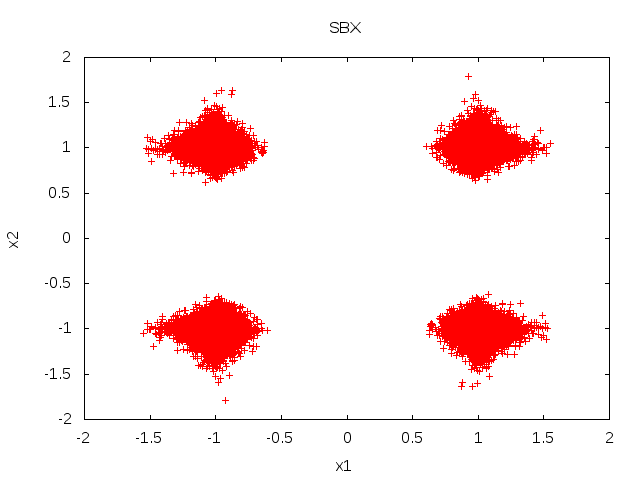
\includegraphics[width=0.35\textwidth]{img/Operadores/SBX_eta_20_2D_pv_1.png} 
   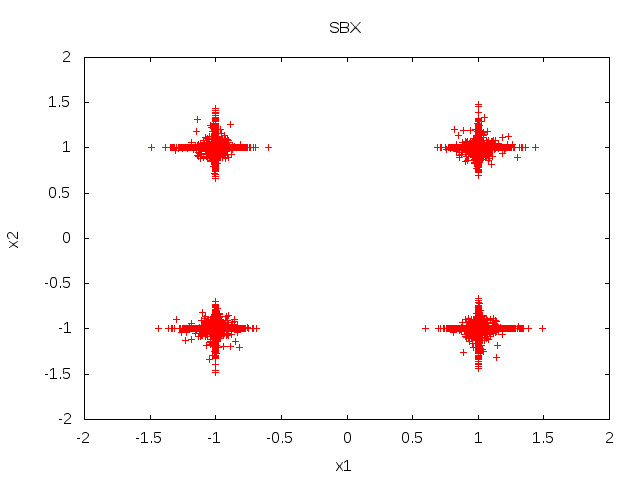
\includegraphics[width=0.35\textwidth]{img/Operadores/SBX_eta_20_2D_pv_01.png} 
\end{tabular}
\caption{Simulaciones de operador \SBX{} con un índice de distribución de $20$. Las soluciones padre están ubicadas en $P_1=(-1.0, -1.0)$ y $P_2=(1.0, 1.0)$. En la parte izquierda la simulación consiste en alterar una variable con probabilidad de $1.0$ y en la pare derecha con probabilidad de $0.1$ (parámetro $\delta_1$ en el Algoritmo \ref{alg:SBX_Operator}).}
\label{fig:Simulation_pv}
\end{figure}



%
\begin{figure}[!t]
\centering
\begin{tabular}{cc}
   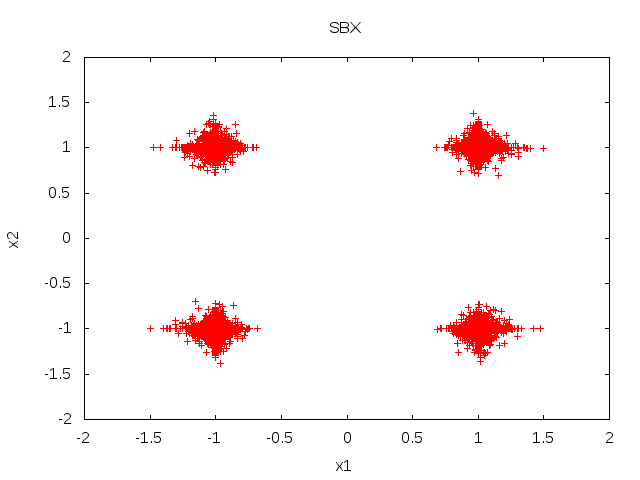
\includegraphics[width=0.35\textwidth]{img/Operadores/SBX_eta_20_2D.png} 
   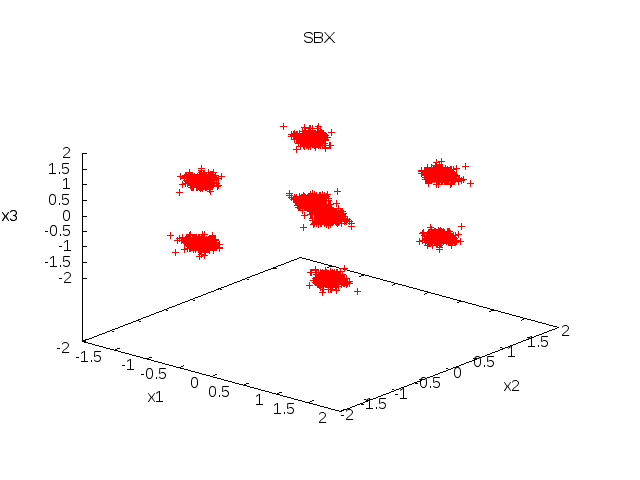
\includegraphics[width=0.35\textwidth]{img/Operadores/SBX_eta_20_3D.png} 
\end{tabular}
\caption{Simulaciones del operador \SBX{} con un índice de distribución de $20$. Las soluciones padre están ubicadas en $P_1=(-1.0, -1.0)$, $P_2=(1.0, 1.0)$ (parte izquierda) y $P_1=(-1.0, -1.0, -1.0)$, $P_2=(1.0, 1.0, 1.0)$ (parte derecha).}
\label{fig:Simulations_Index_20}
\end{figure}


\subsection{Operadores de cruce}

Los operadores de cruce son utilizados para generar soluciones hijas utilizando la información de las soluciones padre.
%
Así, estos operadores combinan las características de dos o más soluciones padre con el propósito de generar nuevas soluciones candidatas.
%
En base a que en la literatura existen diversos operadores de cruce, se han propuesto varias taxonomías para clasificarlos.
%
Particularmente, las taxonomías se basan en varias características tales como la ubicación relativa entre padres e hijos o el tipo 
de relaciones que existen en las variables.

Una clasificación popular hace distinción entre operadores de cruce \textit{basados en las variables} y \textit{basados en los vectores}.
%
En los \textit{basados en las variables}, cada variable de las soluciones padre son combinadas para crear nuevos valores de forma independiente, siendo ideales para
lidiar con problemas separables.
%
Algunos operadores que pertenecen a esta categoría son el \textit{Operador de Cruce por Mezcla} (the Blend Crossover - \BLX{})~\cite{eshelman1993real} 
y el \SBX~\cite{Joel:SBX1994}.
%
Por otra parte, los operadores de recombinación \textit{basados en vectores} tienen en cuenta la relación que existe entre las variables, por lo que
la combinación no es independiente.
%
Así, este tipo de operadores pueden por ejemplo, realizar combinaciones lineales de las soluciones involucradas.
%
Algunos operadores que pertenecen a esta categoría son el \textit{Operador de Cruce Unimodal Normalmente Distribuido} (Unimodal Normally Distributed Crossover - \UNDX{})~\cite{Joel:UNDX}, 
y el \textit{Operador de Cruce Simplex} (Simplex Crossover - \SPX{})~\cite{Joel:DE_Storn_SPX}.
%
Adicionalmente, los operadores de cruce pueden ser clasificados como \textit{centrados en los padres} y \textit{centrados en la media} \cite{jain2011parent}.
%
En los operadores basados en los padres, las soluciones hijas tienden a ser creadas alrededor de cada solución padre, mientras que en los operadores basados 
en la media se tiende a crear a las soluciones hijas alrededor de la media de los valores de las soluciones padres.

\subsubsection{El operador de cruce basado en simulación binaria - SBX}

Entre los operadores de cruce, el \textit{Operador de Cruce Basado en Simulación Binaria} (Simulated Binary Crossover - \SBX{})~\cite{deb1994simulated}
es uno de los más utilizados en dominios continuos y fue el que se decidió extender en nuestra propuesta, por lo que esta sección se centra en este operador de cruce.
%
El operador \SBX{} es clasificado con un operador centrado en los padres, por lo que los valores asociados a los hijos ($c_1$ y $c_2$) serán cercanos a 
los valores de los padres ($p_1$ y $p_2$).
%
Específicamente, el proceso para generar los valores de las soluciones hijo se basa en utilizar una distribución de probabilidad.
%
Esta distribución controla el factor de dispersión $\beta = |c_1 - c_2 | / |p_1 - p_2|$, el cual es definido como la razón entre la distancia de los valores de las soluciones hijas
y la distancia entre los valores de las soluciones padre.
%
Esta función de densidad se define en base a un índice de distribución $\eta_c$ (es un parámetro de control especificado por el usuario) 
el cual altera la capacidad de exploración.
%
Específicamente, un índice pequeño induce una probabilidad elevada de crear valores de las soluciones hijas distantes de los valores de las 
soluciones padre, mientras que índices elevados tienden a crear soluciones muy similares a las soluciones padre, lo cual se ilustra
en la Figura~\ref{fig:fig_sim}.
%
La definición matemática de la distribución y la forma de generar los valores de las soluciones hijas pueden ser estudiados en~\cite{deb1994simulated}.
%
Las ecuaciones iniciales fueron formuladas en base a un problema de optimización sin límites en las variables.
%
Sin embargo, en muchos problemas cada variable está limitada dentro de un límite inferior y superior.
%
Para considerar los límites del espacio de decisión se propuso una modificación de la distribución de probabilidad~\cite{deb1999self}, 
que es la que se usa en este artículo.
%
Para el caso de nuestro método, no es demasiado importante conocer la fórmula exacta, sino el efecto del valor $\eta_c$ que se ha ilustrado previamente.


%Thus, the modification of the probability distribution shown in Equation~(\ref{eq:sbx_spread}) 
%was proposed~\cite{deb1999self} with the aim of taking into account such bounds.
%
%Es importante resaltar que esta última variante es una de las más utilizadas.



%De forma más específica, en el \SBX{} para crear una solución hija se utiliza una distribución de probabilidad que está en función de $\beta \in [0, \infty]$ 
%de la siguiente forma:
%%
%\begin{equation}
%    P(\beta)= 
%\begin{cases}
%     0.5(\eta_c + 1)\beta^{\eta_c},& \text{si} \quad \beta \leq 1\\
%     0.5(\eta_c + 1) \frac{1}{\beta^{\eta_c + 2}} ,& \text{de otra forma}
%\end{cases}
%\end{equation}

%El \SBX{} tiene las siguientes características:
%\begin{itemize}
%\item Los valores de las soluciones hijo son equidistantes de los valores de las soluciones padre.
%\item Existe una probabilidad no nula de crear soluciones hijo en el espacio factible entero por cualquier par de soluciones padre.
%\item La probabilidad general de crear un par de soluciones hijo dentro del rango de las soluciones padre es idéntico a la probabilidad general de crear un par de soluciones hijo fuera del rango de las soluciones padre.
%\end{itemize}

%Por lo tanto, considerando dos valores de las soluciones padre ($p_1$ y $p_2$) se pueden crear dos valores de las soluciones hijo ($c_1$ y $c_2$) en base a una combinación lineal de los valores de las soluciones padre y con un número aleatorio uniforme $u \in [0, 1]$, especificado a continuación:
%Therefore, considering two participating parent values ($p_1$ and $p_2$), two offspring values ($c_1$ and $c_2$) can be created as linear combination of parent values with a uniform random number $u \in [0, 1]$, as follows:
%\begin{equation} 
%\begin{split}
%c_1 &= 0.5(1 + \beta(u))p_1 + 0.5(1 - \beta(u)) p_2 \\
%c_2 &= 0.5(1 - \beta(u))p_1 + 0.5(1 + \beta(u)) p_2
%\end{split}
%\end{equation}

%El parámetro $\beta(u)$ depende en el número aleatorio $u$ de la siguiente forma:
%The parameter $\beta(u)$ depends on the random number $u$, as follows:
%\begin{equation}
%    \beta(u)= 
%\begin{cases}
%     (2u)^{\frac{1}{\eta_c+1}},& \text{si} \quad u \leq 0.5,\\
%     	(\frac{1}{2(1-u)})^{\frac{1}{\eta_c +1}} ,& \text{de otra forma}
%\end{cases}
%\end{equation}

%La ecuación anterior es formulada en base a un problema de optimización sin límites en las variables.
%The above equation considers an optimization problem with no variable bounds.
%
%Sin embargo, en problemas prácticos cada variable es limitada dentro de un límite inferior y superior.
%In most practical problems, each variable is bounded within a lower and upper bound.
%
%Por lo tanto, para considerar los límites del espacio de decisión ~\cite{deb1999self} propusieron una modificación de la distribución de probabilidad en la Ecuación (\ref{eq:sbx_spread}).
%Thus, the modification of the probability distribution shown in Equation~(\ref{eq:sbx_spread}) 
%was proposed~\cite{deb1999self} with the aim of taking into account such bounds.
%
%Es importante resaltar que esta última variante es una de las más utilizadas.
%This last variant is extensively used nowadays.

%
%\begin{equation} \label{eq:sbx_spread}
%    \beta(u)= 
%\begin{cases}
%     (2u(1-\gamma))^{\frac{1}{\eta_c+1}},& \text{si} \quad u \leq 0.5/(1-\gamma),\\
%     	(\frac{1}{2(1-u(1-\gamma))})^{\frac{1}{\eta_c +1}} ,& \text{de otra forma}
%\end{cases}
%\end{equation}
%\begin{equation} \label{eq:child_1}
%c_1 = 0.5(1 + \beta(u))p_1 + 0.5(1-\beta(u))p_2
%\end{equation}
%\begin{equation} \label{eq:child_2}
%c_2 = 0.5(1 + \beta(u))p_1 + 0.5(1-\beta(u))p_2
%\end{equation}

%En este caso, mediante la Ecuación (\ref{eq:child_1}) se calcula el valor de la solución hijo $c_1$ la cual está más cercana a $p_1$.
%In this case, the child $c_1$ which is nearest to $p_1$ is calculated according to the Equation (\ref{eq:child_1}).
%
%Considerando que $p_1 < p_2$ y además con un límite inferior igual a $a$, se tiene que $\gamma = 1/(\alpha^{\eta_c + 1})$, donde $\alpha = 1 + (p_1 - a) / (p_2 - p_1)$.
%Considering that $p_1 < p_2$ and with a lower bound equal to $a$, $\gamma = 1/(\alpha^{\eta_c + 1})$, where $\alpha = 1 + (p_1 - a) / (p_2 - p_1)$.
%
%Similarmente, el segundo valor de la solución hijo $c_2$ se calcula con $\alpha = 1 + (b-p_2)/(p_2 - p_1)$, donde $b$ corresponde al límite superior.
%Similarly, the second child $c_2$ is computed with $\alpha = 1 + (b-p_2)/(p_2 - p_1)$, where $b$ correspond to the upper bound.
%
%Entonces, el segundo valor de la solución hijo se calcula como se indica en la Ecuación (\ref{eq:child_2}).
%Then, the second child is computed as is indicated in Equation (\ref{eq:child_2}).

\begin{algorithm}[t]
\algsetup{linenosize=\tiny}
\scriptsize
\caption{Operador de Cruce basado en Simulación Binaria (\SBX{})}
%\caption{Simulated Binary Crossover (\SBX{})}
\label{alg:SBX_Operator}
\begin{algorithmic}[1]
    \STATE Entrada: Soluciones padre ($P_{1}, P_{2}$), Índice de distribución ($\eta_c$), Probabilidad de cruce ($P_c$).
    %\STATE Input: Parents ($P_{1}, P_{2}$), Distribution index ($\eta_c$), Crossover probability ($P_c$).
    \STATE Salida: Soluciones hijo ($C_{1}, C_{2}$).
    %\STATE Output: Children ($C_{1}, C_{2}$).
    \IF{ $U[0, 1] \leq P_c$}
       \FOR{para cada variable $d$}
       %\FOR{ each variable d}
	\IF{ $U[0, 1] \leq  \delta_1$} \label{alg:inherit_variable}
		\STATE Generar $C_{1,d}$ utilizando las distribuciones dadas en la Ecuación~(\cite{deb1999self}). 
		%\STATE Generate $C_{1,d}$ with Equations (\ref{eq:sbx_spread}) and (\ref{eq:child_1}).
		\STATE Generar $C_{2,d}$ utilizando las distribuciones dadas en la Ecuación~(\cite{deb1999self}).
		%\STATE Generate $C_{1,d}$ with Equations (\ref{eq:sbx_spread}) and (\ref{eq:child_1}).
		 \IF{$ U[0, 1]  \leq  (1 - \delta_2) $} 
			\STATE Intercambiar $C_{1,d}$ con $C_{2,d}$.
		 \ENDIF
        \ELSE
	   \STATE $C_{1,d} = P_{1, d}$.
	   \STATE $C_{2,d} = P_{2, d}$.
        \ENDIF
       \ENDFOR
    \ELSE
	\STATE $C_{1} = P_{1}$.
	\STATE $C_{2} = P_{2}$.
    \ENDIF
\end{algorithmic}
\end{algorithm}

Es importante aclarar que la primer versión del \SBX{} fue diseñada en base a una sola variable.
%
Posteriormente los autores consideraron aplicarlo a problemas con múltiples variables~\cite{Joel:SBX1994}, considerando
una estrategia simple para escoger las variables que se van a cruzar~\cite{Joel:UNDX}.
%
Específicamente, en base a los principios del operador de cruce uniforme, cada variable es cruzada con una probabilidad igual a $0.5$.
%
A pesar de su sencillez y de no tener en cuenta las posibles dependencias entre variables, hoy en día esta es la forma más común de 
aplicar el \SBX{}.

\subsubsection{Implementación y análisis del operador \SBX{}}

En este apartado se discuten algunas de las principales características de la implementación más utilizada del operador \SBX{} para problemas con
múltiples variables.
%
Esencialmente, se consideran tres componentes clave que podrían afectar al rendimiento de los \MOEAS{}.
%
En primer lugar, como ya se mencionó anteriormente, cada variable es alterada con una probabilidad fija igual a $0.5$.
%
Si este valor de probabilidad se incrementa entonces los hijos tienden a crearse a mayor distancia de los padres debido a que se 
modifican más variables de forma simultanea.
%
En los problemas separables, en general interesa modificar sólo una variable mientras que en los no separables suele ser más conveniente
modificar varias variables a la vez.
%
En la Figura~\ref{fig:Simulation_pv} se pueden observar las implicaciones de modificar esta probabilidad considerando un problema con dos variables.
%
Particularmente, en la parte derecha se muestra que una probabilidad pequeña provoca que algunos valores permanezcan intactos, es decir,
hay una tendencia de generar desplazamientos paralelos a los ejes, lo cual suele ser ideal para problemas separables.
%
Por otra parte, en la parte izquierda se muestra que utilizando una probabilidad elevada existe un comportamiento de búsqueda distinto donde la tendencia anterior desaparece, 
lo cual podría ser oportuno para problemas no separables.
%
Es importante destacar que existe una relación entre esta probabilidad y el índice de distribución, ya que estos dos factores tienen un efecto directo en la similitud 
que existe entre las soluciones padres e hijas.
%
\begin{figure}[t]
\centering
\begin{tabular}{c}
   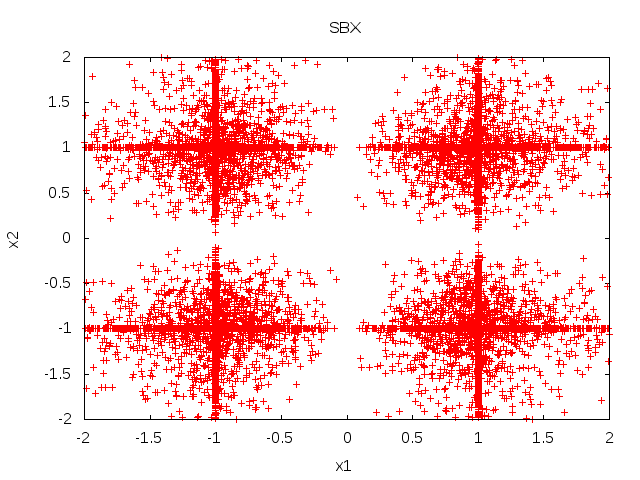
\includegraphics[width=0.35\textwidth]{img/Operadores/SBX_eta_2.png}  %&
   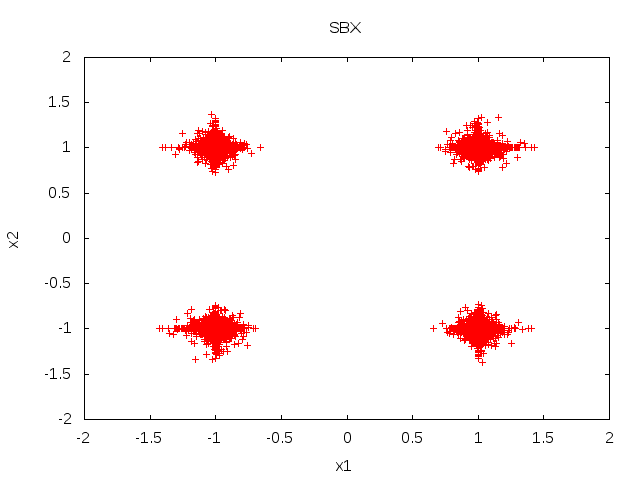
\includegraphics[width=0.35\textwidth]{img/Operadores/SBX_eta_20.png} 
\end{tabular}
\caption{Simulación del operador \SBX{} donde las soluciones padre están ubicadas en $P_1=(-1.0, -1.0)$ y $P_2=(1.0, 1.0)$. En la parte izquierda se consideró un índice de distribución de $2$ y en la derecha de $20$.}
\label{fig:Simulation_Case_3}
\end{figure}

El segundo aspecto importante es que después de generar los dos valores de las soluciones hijas, éstos valores son intercambiados con una probabilidad fija 
(usualmente es $0.5$), es decir el valor de la solución hijo $c_1$ no siempre es heredado a partir de la solución padre más cercana $p_1$.
%
Esta es una característica no muy discutida, sin embargo es un aspecto muy relevante que afecta al rendimiento del algoritmo.
%
En algunos contextos esta probabilidad se denomina ``Probabilidad de cruce uniforme por variable'' (Variable uniform crossover probability) \cite{tuvsar2007differential} 
o ``Recombinación Discreta'' (Discrete Recombination) \cite{muhlenbein1993predictive}.

Dado que en el ámbito multi-objetivo se promueve más diversidad en las variables de decisión de forma implícita, estos intercambios podrían ser altamente disruptivos.
%
De hecho, debido a esto, no es totalmente claro que el \SBX{} deba ser categorizado como un operador centrado en los padres.
%
Estos intercambios que existen entre los valores de las soluciones hijo tienen un efecto de realizar múltiples ``reflexiones'' en el espacio de búsqueda.
%
Así, conforme se incrementa la dimensionalidad en el espacio de las variables, el número de regiones cubiertas crece de forma exponencial como se puede observar en 
los casos de dos y tres dimensiones en la Figura \ref{fig:Simulations_Index_20}.
%
Es importante notar que esta característica tiene un efecto relevante en la distancia entre las soluciones padre y las soluciones hijas.

Finalmente, se discute el índice de distribución que es quizás la característica mas conocida del operador \SBX{}.
%
Un índice de distribución pequeño provoca un grado de exploración elevado.
%
De hecho, un índice de distribución igual a uno tiene un efecto similar al \textit{Operador de Recombinación Difusa} (Fuzzy Recombination Operator)~\cite{voigt1995fuzzy}.
%
En la Figura~\ref{fig:Simulation_Case_3} se puede observar el efecto de aplicar distintos índices de distribución.
%
Particularmente, en la parte izquierda se considera un índice de distribución pequeño, mientras en la parte derecha se considera un índice de distribución grande.
%
Se observa que este último genera soluciones candidatas similares a las soluciones padre.

En el Algoritmo \ref{alg:SBX_Operator} se muestra la implementación del operador \SBX{}.
%The \SBX{} implementation is shown in Algorithm \ref{alg:SBX_Operator}.
%
Este pseudocódigo está basado en la implementación que está integrada en el código del \NSGAII{} propuesto por Deb et al.~\cite{Joel:NSGAII}, 
la cual se considera como la variante más popular.
%
En los parámetros de entrada se requieren dos soluciones padre ($P_1$, $P_2$), y éste crea dos soluciones hijas ($C_1$, $C_2$).
%
El primero y el segundo componente mencionados previamente corresponden a las líneas 5 y 9 respectivamente.
%
El caso clásico del operador \SBX{} se configura con los parámetros $\delta_1 = \delta_2 = 0.5$ y $\eta_c = 20$.
%
Es importante hacer notar que la implementación clásica no considera la dimensionalidad de las variables o el criterio de paro como parte de sus parámetros internos.

\subsection{Propuesta - \DSBX{}}

Basado en el análisis anterior y con el propósito de inducir un balanceo entre exploración e intensificación de forma dinámica y que dependa del instante de ejecución, 
se proponen las siguiente modificaciones.
%
En primer lugar, se modifica la probabilidad de alterar una variable ($\delta_1$) durante la ejecución.
%
La intención de esta modificación es estimular la capacidad de exploración considerando inicialmente una probabilidad elevada 
para alterar más variables de forma simultánea, mientras que conforme la ejecución avanza se reduce esta probabilidad, con el fin de reducir
el número de variables que se modifican y promover así movimientos más pequeños.
%
El valor de $\delta_1$ se cambia en base a un modelo lineal decreciente, donde inicialmente se fija a $1.0$ y se decrementa de forma
que a la mitad del total de generaciones alcanza el valor $0.5$.
%
Este último valor es mantenido hasta el final de la ejecución, es decir, desde la mitad de la ejecución este parámetro se fija 
al mismo valor que el de la implementación tradicional del \SBX{}.
%
Para asignar el valor $\delta_1$ se utiliza la Ecuación (\ref{eqn:linear}), donde $G_{Transcurridas}$ corresponde a la generación actual 
y $G_{Total}$ corresponde al número total de generaciones.

El segundo cambio está relacionado con la probabilidad de aplicar reflexiones ($1 - \delta_2$).
%
En este caso $\delta_2$ es actualizado de acuerdo a la Ecuación (\ref{eqn:linear}), por lo tanto la probabilidad de aplicar una reflexión 
incrementa de $0.0$ a $0.5$ durante la ejecución.
%
Esta modificación se realiza con el propósito de evitar el comportamiento disruptivo de intercambiar variables en las primeras generaciones 
ya que esto provocaría modificaciones muy drásticas.
%
De esta forma, sería mas sensato aplicar estas reflexiones una vez que los individuos convergen en cierto grado.
%
Nótese que se incrementa hasta el valor $0.5$ el cual es el valor utilizando en la implementación del \SBX{} estándar, ya que no se quiere
disponer de un comportamiento excesivamente disruptivo.
%
Sin embargo, en el futuro sería interesante realizar estudios con otros valores finales.

\begin{equation}\label{eqn:linear}
	\delta_1 = \delta_2 = max \left (0.5, 1.0 - \frac{G_{Transcurridas}}{G_{Total}} \right )
\end{equation}

Finalmente, el índice de distribución también es modificado durante la ejecución.
%
En las primeras etapas se promueve un índice de distribución pequeño con el propósito de incrementar la capacidad de exploración del \SBX{}.
%
Posteriormente se decrementa de forma lineal, lo cual tiene el efecto de que la curva de distribución se cierre, y por lo tanto se promueve 
un mayor grado de intensificación en las etapas finales.
%
El incremento lineal es llevado a cabo usando la Ecuación (\ref{eqn:index_eta}), por lo tanto el índice de distribución es alterado de $2$ a $22$.
%
Es importante aclarar que ya se han considerado modificaciones similares al índice de distribución \cite{zitzler1999multiobjective}, \cite{hamdan2012distribution},
aunque las otras propiedades que se modifican nunca han sido estudiadas en profundidad.

\begin{equation}\label{eqn:index_eta}
 \eta_c = 2 + 20 \times \left ( \frac{G_{Transcurridas}}{G_{Total}} \right)
\end{equation}

\subsection{Resultados}

\begin{table}[t]
\centering
\caption{Puntos de referencias para el indicador HV}
%\caption{References points for the HV indicator}
\label{tab:ReferencePoints}
\begin{scriptsize}
\begin{tabular}{cc}
\hline
\textbf{Instancias} & \textbf{Punto de referencia} \\ \hline
%\textbf{Instances} & \textbf{Reference Point} \\ \hline
WFG1-WFG9 & $[2.1, ...,2m+0.1]$ \\
DTLZ 1, 2, 4 & $[1.1, ..., 1.1]$ \\
DTLZ 3, 5, 6 & $[3, ..., 3]$ \\
DTLZ7 & $[1.1, ..., 1.1, 2m]$ \\
UF 1-10 & $[2, ..., 2]$ \\ \hline
\end{tabular}
\end{scriptsize}
\end{table}


% Please add the following required packages to your document preamble:
% \usepackage{multirow}
% \usepackage{graphicx}
\begin{table*}[t]
\centering

\caption{Información estadística de las métricas considerando dos objetivos}
%\caption{Statistical Information of Metrics with two objectives}
\label{tab:Metrics_2}
\resizebox{\textwidth}{!}{%
\begin{tabular}{|c|c|c|c|c|c|c|c|c|c|c|c|c|c|c|c|c|c|c|}
\hline
\multirow{2}{*}{} & \multicolumn{6}{c|}{NSGA-II} & \multicolumn{6}{c|}{MOEA/D} & \multicolumn{6}{c|}{SMS-EMOA} \\ \cline{2-19} 
 & 1 & 2 & 3 & 4 & 5 & DE & 1 & 2 & 3 & 4 & 5 & DE & 1 & 2 & 3 & 4 & 5 & DE \\ \hline
Average HV & 0.88 & 0.90 & 0.90 & 0.91 & 0.93 & \textbf{0.94} & 0.87 & 0.87 & 0.87 & 0.90 & \textbf{0.91} & \textbf{0.91} & 0.88 & 0.89 & 0.87 & 0.91 & 0.92 & \textbf{0.93} \\ \hline
%Best Counts HV & 2 & 1 & 0 & 1 & 8 & \textbf{11} & 2 & 0 & 2 & 2 & 8 & \textbf{9} & 0 & 1 & 1 & 5 & 6 & \textbf{10} \\ \hline
%\multicolumn{1}{|l|}{Average Best Difference HV} & \multicolumn{1}{l|}{0.068} & \multicolumn{1}{l|}{0.057} & \multicolumn{1}{l|}{0.053} & \multicolumn{1}{l|}{0.039} & \multicolumn{1}{l|}{0.019} & \multicolumn{1}{l|}{\textbf{0.017}} & \multicolumn{1}{l|}{0.053} & \multicolumn{1}{l|}{0.048} & \multicolumn{1}{l|}{0.049} & \multicolumn{1}{l|}{0.024} & \multicolumn{1}{l|}{\textbf{0.013}} & \multicolumn{1}{l|}{0.014} & \multicolumn{1}{l|}{0.074} & \multicolumn{1}{l|}{0.064} & \multicolumn{1}{l|}{0.081} & \multicolumn{1}{l|}{0.045} & \multicolumn{1}{l|}{0.028} & \multicolumn{1}{l|}{\textbf{0.019}} \\ \hline
Average IGD+ & 0.12 & 0.09 & 0.11 & 0.07 & 0.06 & \textbf{0.05} & 0.14 & 0.12 & 0.14 & 0.09 & 0.08 & \textbf{0.07} & 0.13 & 0.11 & 0.14 & 0.08 & 0.07 & \textbf{0.05} \\ \hline
%Best Counts IGD+ & 2 & 1 & 1 & 1 & 8 & \textbf{10} & 3 & 0 & 2 & 3 & 6 & \textbf{9} & 0 & 2 & 0 & 3 & \textbf{9} & \textbf{9} \\ \hline
%\multicolumn{1}{|l|}{Average Best Difference IGD+} & \multicolumn{1}{l|}{0.086} & \multicolumn{1}{l|}{0.052} & \multicolumn{1}{l|}{0.077} & \multicolumn{1}{l|}{0.035} & \multicolumn{1}{l|}{0.021} & \multicolumn{1}{l|}{\textbf{0.016}} & \multicolumn{1}{l|}{0.075} & \multicolumn{1}{l|}{0.059} & \multicolumn{1}{l|}{0.072} & \multicolumn{1}{l|}{0.025} & \multicolumn{1}{l|}{0.019} & \multicolumn{1}{l|}{\textbf{0.008}} & \multicolumn{1}{l|}{0.093} & \multicolumn{1}{l|}{0.071} & \multicolumn{1}{l|}{0.101} & \multicolumn{1}{l|}{0.038} & \multicolumn{1}{l|}{0.030} & \multicolumn{1}{l|}{\textbf{0.017}} \\ \hline
\end{tabular}%
}
\end{table*}

% Please add the following required packages to your document preamble:
% \usepackage{multirow}
% \usepackage{graphicx}
\begin{table*}[t]
\centering
\caption{Información estadística de las métricas considerando tres objetivos}
%\caption{Statistical Information of Metrics with three objectives}
\label{tab:Metrics_3}
\resizebox{\textwidth}{!}{%
\begin{tabular}{|c|c|c|c|c|c|c|c|c|c|c|c|c|c|c|c|c|c|c|}
\hline
\multirow{2}{*}{} & \multicolumn{6}{c|}{NSGA-II} & \multicolumn{6}{c|}{MOEA/D} & \multicolumn{6}{c|}{SMS-EMOA} \\ \cline{2-19} 
 & 1 & 2 & 3 & 4 & 5 & DE & 1 & 2 & 3 & 4 & 5 & DE & 1 & 2 & 3 & 4 & 5 & DE \\ \hline
Average HV & \textbf{0.87} & 0.84 & \textbf{0.87} & \textbf{0.87} & \textbf{0.87} & 0.85 & 0.84 & 0.84 & 0.84 & \textbf{0.86} & \textbf{0.86} & 0.85 & 0.90 & 0.89 & 0.88 & \textbf{0.91} & \textbf{0.91} & \textbf{0.91} \\ \hline
%Best Counts HV & 1 & 2 & 1 & 4 & 4 & \textbf{7} & 1 & 2 & 1 & 2 & 5 & \textbf{8} & 3 & 2 & 0 & 2 & 5 & \textbf{7} \\ \hline
%\multicolumn{1}{|l|}{Average Best Difference HV} & \multicolumn{1}{l|}{0.019} & \multicolumn{1}{l|}{0.047} & \multicolumn{1}{l|}{0.020} & \multicolumn{1}{l|}{\textbf{0.014}} & \multicolumn{1}{l|}{\textbf{0.014}} & \multicolumn{1}{l|}{0.032} & \multicolumn{1}{l|}{0.036} & \multicolumn{1}{l|}{0.041} & \multicolumn{1}{l|}{0.038} & \multicolumn{1}{l|}{0.016} & \multicolumn{1}{l|}{\textbf{0.013}} & \multicolumn{1}{l|}{0.027} & \multicolumn{1}{l|}{0.038} & \multicolumn{1}{l|}{0.038} & \multicolumn{1}{l|}{0.049} & \multicolumn{1}{l|}{\textbf{0.019}} & \multicolumn{1}{l|}{0.027} & \multicolumn{1}{l|}{\textbf{0.019}} \\ \hline
Average IGD+ & 0.13 & 0.16 & 0.13 & \textbf{0.12} & \textbf{0.12} & 0.13 & 0.15 & 0.14 & 0.15 & \textbf{0.11} & \textbf{0.11} & 0.13 & 0.11 & 0.11 & 0.13 & \textbf{0.09} & \textbf{0.09} & 0.13 \\ \hline
%Best Counts IGD+ & 0 & 2 & 2 & 4 & 3 & \textbf{8} & 2 & 2 & 0 & 2 & 4 & \textbf{9} & 1 & 3 & 0 & 3 & 5 & \textbf{7} \\ \hline
%\multicolumn{1}{|l|}{Average Best Difference IGD+} & \multicolumn{1}{l|}{0.029} & \multicolumn{1}{l|}{0.061} & \multicolumn{1}{l|}{0.027} & \multicolumn{1}{l|}{0.023} & \multicolumn{1}{l|}{\textbf{0.020}} & \multicolumn{1}{l|}{0.032} & \multicolumn{1}{l|}{0.053} & \multicolumn{1}{l|}{0.048} & \multicolumn{1}{l|}{0.053} & \multicolumn{1}{l|}{\textbf{0.015}} & \multicolumn{1}{l|}{\textbf{0.015}} & \multicolumn{1}{l|}{0.030} & \multicolumn{1}{l|}{0.047} & \multicolumn{1}{l|}{0.040} & \multicolumn{1}{l|}{0.062} & \multicolumn{1}{l|}{\textbf{0.020}} & \multicolumn{1}{l|}{0.024} & \multicolumn{1}{l|}{0.069} \\ \hline
\end{tabular}%
}
\end{table*}
\begin{table*}[t]
\centering
\caption{Resumen de las pruebas estadísticas}
%\caption{Summary of Statistical Tests}
\label{tab:statistical_Tests}
\begin{scriptsize}
\begin{tabular}{|c|c|c|c|c|c|c|c|c|c|c|c|c|c|c|c|}
\hline
\multicolumn{16}{|c|}{NSGA-II} \\ \hline
 & \multicolumn{3}{c|}{1} & \multicolumn{3}{c|}{2} & \multicolumn{3}{c|}{3} & \multicolumn{3}{c|}{4} & \multicolumn{3}{c|}{5} \\ \hline
 & $\uparrow$ & $\downarrow$ & $\longleftrightarrow$ & $\uparrow$ & $\downarrow$ & $\longleftrightarrow$ & $\uparrow$ & $\downarrow$ & $\longleftrightarrow$ & $\uparrow$ & $\downarrow$ & $\longleftrightarrow$ & $\uparrow$ & $\downarrow$ & $\longleftrightarrow$ \\ \hline
\textbf{HV-2obj} & 16 & 29 & 47 & 6 & 61 & 25 & 28 & 19 & 45 & 31 & 23 & 38 & \textbf{54} & 3 & 35 \\ \hline
\textbf{HV-3obj} & 15 & 19 & 42 & 12 & 50 & 14 & 17 & 15 & 44 & \textbf{33} & 10 & 33 & 26 & 9 & 41 \\ \hline
\textbf{IGD-2obj} & 14 & 30 & 48 & 4 & 60 & 28 & 25 & 17 & 50 & 33 & 19 & 40 & \textbf{52} & 2 & 38 \\ \hline
\textbf{IGD-3obj} & 14 & 18 & 44 & 13 & 44 & 19 & 18 & 15 & 43 & \textbf{33} & 15 & 28 & 23 & 9 & 44 \\ \hline
% \end{tabular}
% \end{table*}

% \begin{table*}[]
% \centering
% \caption{My caption}
% \label{my-label}
% \begin{tabular}{|c|c|c|c|c|c|c|c|c|c|c|c|c|c|c|c|}
\hline
\hline
\multicolumn{16}{|c|}{MOEA/D} \\ \hline
 & \multicolumn{3}{c|}{1} & \multicolumn{3}{c|}{2} & \multicolumn{3}{c|}{3} & \multicolumn{3}{c|}{4} & \multicolumn{3}{c|}{5} \\ \hline
 & $\uparrow$ & $\downarrow$ & $\longleftrightarrow$ & $\uparrow$ & $\downarrow$ & $\longleftrightarrow$ & $\uparrow$ & $\downarrow$ & $\longleftrightarrow$ & $\uparrow$ & $\downarrow$ & $\longleftrightarrow$ & $\uparrow$ & $\downarrow$ & $\longleftrightarrow$ \\ \hline
\textbf{HV-2obj} & 15 & 33 & 44 & 10 & 60 & 22 & 25 & 26 & 41 & 39 & 18 & 35 & \textbf{57} & 9 & 26 \\ \hline
\textbf{HV-3obj} & 10 & 22 & 44 & 12 & 39 & 25 & 11 & 19 & 46 & 24 & 10 & 42 & \textbf{38} & 5 & 33 \\ \hline
\textbf{IGD-2obj} & 16 & 31 & 45 & 9 & 60 & 23 & 23 & 27 & 42 & 37 & 17 & 38 & \textbf{57} & 7 & 28 \\ \hline
\textbf{IGD-3obj} & 12 & 22 & 42 & 13 & 43 & 20 & 13 & 24 & 39 & 30 & 9 & 37 & \textbf{40} & 10 & 26 \\ \hline
% \end{tabular}
% \end{table*}

% \begin{table*}[]
% \centering
% \caption{My caption}
% \label{my-label}
% \begin{tabular}{|c|c|c|c|c|c|c|c|c|c|c|c|c|c|c|c|}
\hline
\hline
\multicolumn{16}{|c|}{SMS-EMOA} \\ \hline
 & \multicolumn{3}{c|}{1} & \multicolumn{3}{c|}{2} & \multicolumn{3}{c|}{3} & \multicolumn{3}{c|}{4} & \multicolumn{3}{c|}{5} \\ \hline
 & $\uparrow$ & $\downarrow$ & $\longleftrightarrow$ & $\uparrow$ & $\downarrow$ & $\longleftrightarrow$ & $\uparrow$ & $\downarrow$ & $\longleftrightarrow$ & $\uparrow$ & $\downarrow$ & $\longleftrightarrow$ & $\uparrow$ & $\downarrow$ & $\longleftrightarrow$ \\ \hline
\textbf{HV-2obj} & 9 & 35 & 48 & 7 & 43 & 42 & 16 & 31 & 45 & 41 & 9 & 42 & \textbf{53} & 8 & 31 \\ \hline
\textbf{HV-3obj} & 7 & 21 & 48 & 9 & 35 & 32 & 13 & 21 & 42 & 27 & 6 & 43 & \textbf{31} & 4 & 41 \\ \hline
\textbf{IGD-2obj} & 10 & 34 & 48 & 15 & 48 & 29 & 12 & 33 & 47 & 41 & 12 & 39 & \textbf{55} & 6 & 31 \\ \hline
\textbf{IGD-3obj} & 8 & 20 & 48 & 13 & 30 & 33 & 9 & 19 & 48 & 22 & 5 & 49 & \textbf{27} & 5 & 44 \\ \hline
\end{tabular}
\end{scriptsize}
\end{table*}

En este apartado se analizan los resultados obtenidos con las variantes dinámicas del \SBX{} (\DSBX{}).
%
El nuevo operador de cruce se integró en los algoritmos \NSGAII{}, \MOEAD{} y \SMSEMOA{}.
%
En primer lugar, se analiza cada una de las tres modificaciones propuestas de forma aislada.
%
Posteriormente se construye un caso donde se consideran las dos modificaciones ofrecieron mejores resultados de forma simultánea.
%
Como parte de la validación experimental se consideran los problemas de prueba WFG~\cite{Joel:WFG}, DTLZ~\cite{Joel:DTLZ_2} y UF~\cite{zhang2009performance}.
%
Además, con el propósito de comparar nuestra extensión del \SBX{} con otros operadores se incluye la variante de evolución diferencial conocida como \DEMO{}~\cite{tuvsar2007differential}.

Para llevar a cabo el análisis experimental, y dado que todos los algoritmos son estocásticos, cada caso fue ejecutado $35$ 
veces con distintas semillas.
%
La configuración global que se aplicó a todos los algoritmos fue la siguiente.
%
Se asignó el criterio de paro a $25,000$ generaciones, el tamaño de la población a $100$, 
se configuraron los problemas de prueba \WFG{} con dos y tres objetivos considerando 24 variables, 
donde $20$ variables son parámetros de distancia y $4$ son parámetros de posición.
%
Como es sugerido en~\cite{Joel:DTLZ_2} se consideró $n=M+r-1$ variables de decisión en los problemas de prueba \DTLZ{}, 
donde para los problemas DTLZ1, DTLZ2 - DTLZ6 y DTLZ7 se consideraron $r=\{5, 10, 20\}$  respectivamente.
% 
En el caso de los problemas de prueba \UF{} se utilizaron $10$ variables de decisión.
%
Finalmente, se hizo uso del operador de mutación polinomial con una probabilidad de mutación de $1/n$ y con un índice de distribución igual a $50$, 
mientras que el operador de cruce \SBX{} se utilizó con una probabilidad de cruce igual a $0.9$ y un índice de distribución de $20$.

A continuación se especifica la parametrización adicional propia cada algoritmo:
\begin{itemize}
\item \textbf{DEMO}: CR = 0.3 y F = 0.5.
\item \textbf{SMS-EMOA}: desplazamiento para calcular el HV = 100.
\item \textbf{MOEA/D}: tamaño de la vecindad = 10, el número de actualizaciones por subproblema ($nr$) = 2 y $\delta = 0.9$.
\end{itemize}

Para comparar los frentes obtenidos por cada método se utiliza el hipervolumen normalizado (HV) y la 
\textit{Distancia Generacional Invertida Modificada} (Inverted Generational Distance Plus - IGD+).
%
En la Tabla \ref{tab:ReferencePoints} se presentan los puntos de referencia utilizados para el indicador del hipervolumen los cuales son similares 
a los utilizados en \cite{Joel:Kuhn_Munkres, Joel:OperatorAHX}.
%
Por otra parte para comparar los resultados estadísticamente (valores del IGD+ y HV), se siguió un procedimiento similar al que se propuso en~\cite{Joel:StatisticalTest},
siendo el mismo que se aplicó para validar la primera propuesta.
%In order to statistically compare the results (IGD+ and HV values), the following statistical tests were performed. 
%In order to statistically compare the results, a similar guideline than the one proposed in~\cite{Joel:StatisticalTest} was used. 
%
%En primer lugar, se utilizó la prueba Shapiro-Wilk para comprobar si los resultados se ajustaban a una distribución Gaussiana. 
%
%First a Shapiro-Wilk test was performed to check whatever or not the values of the results followed a Gaussian distribution. 
%
%En los casos en que sí se ajustaban, se utilizó la prueba de Levene para comprobar la homogeneidad de las varianzas, procediendo con la prueba de ANOVA en caso positivo o con el de Welch en caso negativo.
%
%If, so, the Levene test was used to check for the homogeneity of the variances. 
%If samples had equal variance, an ANOVA test was done; if not, a Welch test was performed. 
%
%Por otro lado, para los casos que no se ajustaban a distribuciones Guassianas, se utilizó la prueba de Kruskal-Wallis.
%For non-Gaussian distributions, the nonparametric Kruskal-Wallis test was used to test whether samples are drawn 
%from the same distribution. 
%
%En todos los casos se fijó el nivel de confianza al 95\%.
%
%Se considera que un algoritmo $X$ es superior a un algoritmo $Y$, si el procedimiento anterior reporta diferencias significativas, además si la media y mediana del hipervolumen obtenido por el método $X$ son superiores a las obtenidas por el método $Y$.
%
%An algorithm $X$ is said to win algorithm $Y$ when the differences between them are statistically significant, and
%the mean and median obtained by $X$ are higher (in HV) or lower (in IGD+) than the mean and median achieved by $Y$.


\subsection{Análisis de cada modificación en el operador \SBX{}}

En este apartado se analiza el efecto que cada modificación propuesta tiene de forma independiente sobre los resultados obtenidos.
%
Para ello basados en el Algoritmo \ref{alg:SBX_Operator} se proponen cuatro casos:

\begin{itemize}
\item \textbf{Caso 1}: se aplica la versión estándar del operador \SBX{} donde $\delta_1 = \delta_2 = 0.5$ y $\eta_c = 20$.
\item \textbf{Caso 2}: se actualiza el valor $\delta_1$ como se indica en la Ecuación~(\ref{eqn:linear}),  $\delta_2=0.5$ y $\eta_c = 20$.
\item \textbf{Caso 3}: se actualiza el valor $\delta_2$ como se indica en la Ecuación~(\ref{eqn:linear}), $\delta_1=0.5$ y $\eta_c = 20$.
\item \textbf{Caso 4}: se actualiza el índice de distribución de acuerdo a~(\ref{eqn:index_eta}), $\delta_1=\delta_2=0.5$.
\end{itemize}

En las Tablas \ref{tab:Metrics_2} y \ref{tab:Metrics_3} se muestra información del HV normalizado \cite{zitzler1999multiobjective} y del IGD+ \cite{Joel:IGDPlus_And_GDPlus} para cada caso, con
dos y tres objetivos respectivamente (el Caso 5 se comenta más adelante).
%
Específicamente, se muestra la media del HV e IGD+ para todos los problemas en dos y tres objetivos.
%
Se observa que considerando dos y tres objetivos el Caso 4 mejora al Caso 1, al Caso 2 y al Caso 3 en todos los algoritmos.
%
Por lo tanto se aprecian de forma clara los beneficios de incrementar el índice de distribución durante la ejecución.
%
Por otra parte, al considerar tres objetivos, el Caso 2 presentó un rendimiento menor que al Caso 1, 
posiblemente debido a que al alterar tantas variables de forma simultánea, se produce un comportamiento excesivamente disruptivo.
%
Quizás los resultados podrían mejorar si el parámetro $\delta_1$ es alterado de una forma distinta, sin embargo esto se deja como trabajo futuro.
%
Los análisis anteriores únicamente consideran la media obtenida en todos los problemas de prueba.
%
%Sin embargo, dependiendo en el tipo de problema el rendimiento del algoritmo podría variar, hecho que se analiza en la siguiente sección.
En la Tabla~\ref{tab:statistical_Tests} se muestra los resultados de las pruebas estadísticas (el Caso 5 se discute en la siguiente sección).
%
Particularmente, se realizan comparaciones por pares en base a las pruebas estadísticas ya mencionadas entre los cinco casos.
%
Este procedimiento se realizó de forma independiente para cada el \NSGAII{}, \MOEAD{} y el \SMSEMOA{}.

Para cada algoritmo y para cada caso, la columna ``$\uparrow$'' reporta el número de comparaciones donde las pruebas estadísticas confirmaron 
la superioridad del caso correspondiente, mientras que en la columna ``$\downarrow$'' se reporta el número de veces donde este caso fue inferior 
y la columna ``$\longleftrightarrow$'' indica el número de comparaciones donde la diferencia estadística no fue significativamente distinto.
%
Principalmente se observa que el Caso 3 es superior al Caso 1 y al Caso 2, sin embargo el Caso 3 es peor que el Caso 4, el motivo de esto es que alterar el índice de distribución tiene un impacto considerable en el proceso de búsqueda.
%
Por otra parte, se observa que el Caso 3 es mejor que la versión estándar del operador SBX (Caso 1), además el Caso 2 es peor que el Caso 1.
%
Por lo tanto se puede intuir que las modificaciones impuestas por el Caso 3 y el Caso 4 pueden ser aplicadas de forma simultánea, ya que incrementar el índice de distribución y aumentar el número de veces en que se intercambian los valores hijos induce un balanceo adecuado entre exploración e intensificación de las regiones promisorias.
%
%Además, combinar el Caso 4 y el Caso 2 tendría efectos negativos, esto en base a que se obtuvieron malos resultados considerando únicamente al Caso 2, por lo tanto juntar este último y aumentar el índice de distribución tendrá un comportamiento inestable.
%
Adicionalmente, se anexan resultados detallados para facilitar que otros investigadores puedan realizar comparativas con un mayor
nivel de detalle\footnote{https:\//\//github.com\//joelchaconcastillo\//SBX\_CEC2018.}.


\subsection{Modificación simultánea de varios componentes}

En base a los análisis realizados con anterioridad se propone una variante del operador \SBX{} que incorpora las modificaciones propuestas
en el Caso 3 y Caso 4 de forma simultánea, es decir, se incorpora un cambio dinámico tanto en el parámetro $\delta_2$ como en el índice de distribución.
%
Debido a los resultados de baja calidad del Caso 2 el parámetro $\delta_1$ no se modifica de forma dinámica.
%
Particularmente, el Caso 5 se construye en base al Algoritmo \ref{alg:SBX_Operator} asignando el parámetro $\delta_1$ a $0.5$ debido
a que es la forma de la versión estándar del \SBX{}, mientras que $\delta_2$ es actualizado de acuerdo a la Ecuación~(\ref{eqn:linear}) y
el parámetro $\eta_c$ es actualizado como se indica en la Ecuación (\ref{eqn:index_eta}).

De acuerdo a la media del HV y del IGD+ que se obtuvieron en el Caso 5 (ver Tablas~\ref{tab:Metrics_2} y \ref{tab:Metrics_3}), es claro que integrar los 
Casos 3 y 4 proporciona beneficios importantes.
%
En el caso de dos objetivos se observa una ventaja significativa, sin embargo en el caso de tres objetivo los Casos 4 y 5 son muy similares en base a la media.
%
Además, al considerar tres objetivos los resultados que se obtuvieron en el Caso 5 son superiores a los obtenidos con \DE{}, 
mientras que al considerar la versión estándar de \SBX{} se observa un deterioro.
%
Por lo tanto, si el operador \SBX{} es configurado adecuadamente puede generar resultados similares o superiores que el algoritmo \DEMO{}. 

%Finalmente, se presenta un análisis adicional para comprender mejor las contribuciones de los distintos casos.
%%
%Particularmente, se realizan comparaciones por pares en base a las pruebas estadísticas ya mencionadas entre los cinco casos.
%%
%Este procedimiento se realizó de forma independiente para cada el \NSGAII{}, \MOEAD{} y el \SMSEMOA{}.
%%%%%%%%%%%%%%%%%
%En la Tabla~\ref{tab:statistical_Tests}, se muestra los resultados de las pruebas estadísticas.
%%
%Para cada algoritmo y para cada caso, la columna ``$\uparrow$'' reporta el número de comparaciones donde las pruebas estadísticas confirmaron 
%la superioridad del caso correspondiente, mientras que en la columna ``$\downarrow$'' se reporta el número de veces donde este caso fue inferior 
%y la columna ``$\longleftrightarrow$'' indica el número de comparaciones donde la diferencia estadística no fue significativamente distinto.
%%
Finalmente, en la Tabla~\ref{tab:statistical_Tests}, se muestra los resultados de las pruebas estadísticas.
%
Los beneficios obtenidos por el Caso 5 son muy claros, de hecho,
únicamente el Caso 4 obtuvo mejores resultados que el Caso 5 al considerar tres objetivos y al algoritmo \NSGAII{}.
%
Esto demuestra que se pueden obtener mejores resultados si se integran varias modificaciones dinámicas de forma simultánea.
%
Además, los resultados confirman las ventajas de la versión dinámica frente al caso estándar (Caso 1).
%
El único caso que no presenta ventajas importantes frente a la versión estándar del \SBX{} es el Caso 2, el cual fue discutido con anterioridad.
